%%%
%%% Übersetzen mit:

%%% > biber main
%%% > pdflatex main.tex
%%% > pdflatex main.tex
%%% danach sollte ein main.pdf erzeugt worden sein


\documentclass[
	10pt,			% Standardschrtift
	a4paper,		% Seitengroesse
	%oneside,		% einseitiger Druck
	parskip=half,		% Standard Paragraphformatierung
	DIV=4,			% führt die Satzspiegelberechnung neu aus
	captions=nooneline,	%
	tablecaptionabove,	% Tabellenüberschriften aktivieren
	bibliography=totoc,	% Stil fuer Literaturangaben
	bibtotocnumbered,	% Literaturverzeichnis ins Inhaltsverzeichnis
	liststotocnumbered,	% Alle Listen ins Inhaltsverzeichnis
	headinclude,
	headsepline,		% 
	1.6headlines,		%
	]
	{book}

\usepackage{tikz}
\usepackage{xcolor} % Farben
\usepackage{color, colortbl}
\usetikzlibrary{decorations.pathmorphing}
\usetikzlibrary{decorations.pathreplacing}
\usetikzlibrary{arrows, decorations.markings}
\usepackage{pgfplots}
\usepackage{pstricks-add}
\usepackage{amsmath}
\usepackage{amssymb}
\usepackage{caption}
\usepackage{stix}
\usepackage{booktabs}
\usepackage{nonfloat}
\usepackage{multicol}
\usepackage{tabularx}
\usepackage{url}
\usepackage{longtable}
\usepackage{svg}
\usepackage[onehalfspacing]{setspace}
\usepackage[sfdefault]{noto} % Standardschrift aendern
\usepackage[utf8]{inputenc}
\usepackage{float}
\usepackage[english]{babel} % Woerterbuch
%\usepackage[ngerman]{babel}
\definecolor{tableHeader}{RGB}{255,238,205}
\definecolor{white}{RGB}{255,255,255}
\usepackage[left=2.50cm, right=2.50cm, top=2.50cm, bottom=3.0cm]{geometry} % Seitengeometrie
\newcommand*\circled[1]{\tikz[baseline=(char.base)]{
		\node[shape=circle,draw,inner sep=1pt] (char) {#1};}}
\newcommand{\mline}[1]{\begin{tabular}{@{}l@{}}#1\end{tabular}}
\newcommand\myfigure[1]{%
	\medskip\noindent\begin{minipage}{\columnwidth}
		\centering%
		#1%
		%figure,caption, and label go here
	\end{minipage}\medskip}

%\usepackage[
%backend=biber,
%style=is-unsrt,
%sortlocale=de_DE,
%natbib=true,
%url=false, 
%doi=true,
%eprint=false,
%backref=false %% In den Literaturangaben anzeigen, an welchen Stellen/Seiten das Zitat gesetzt ist
%]{biblatex}
%\addbibresource{test.bib} 
\newcommand{\quotes}[1]{\glqq#1\grqq}


%%%%%%%%%%%%%%%%%%%%
%% Daten anpassen %%
%%%%%%%%%%%%%%%%%%%%

\def\thesisAuthor{Max Mustermann}
\def\thesisTitle{Wahnsinn und Mut}
\def\thesisDate{30. Juni 2018}
\def\thesisType{Bachelor}
\def\thesisContact{mail@mail.com}
\def\thesisMatnr{1231231}
\def\thesisSupervisor{Prof.~Dr.~rer.~nat. Harald Görl}


%%% Trennungen:
\hyphenation{bei-spiels-wei-se}
%%% Bindestrich, der andere Trennungen unterdrückt: -
%%% Bindestrich, der andere Trennungen erlaubt: "=
%%% Bindestrich, an dem nicht getrennt werden darf: "~
%%% Trennmöglichkeit, die andere Trennungen ausschließt: \-


%%% Damit das Design mit Rändern usw. als allererste Seite ausgegeben wird:
\usepackage{layouts}
\setlayoutscale{0.33}
\setparametertextfont{\scriptsize}
\currentpage
%%% Wenn das Design nicht erwünscht ist, weg mit diesen Zeilen



\begin{document}


%%% Design
\pagedesign
\newpage
%%% Wenn das Design nicht erwünscht ist, weg mit diesen beiden Zeilen


%% Titelblatt
\thispagestyle{empty}

% Image
\begin{figure}[t]
	 \centering
	 \includegraphics[width=11.0cm]{unibw.eps}
\end{figure}

% University title 
\begin{center}
	\Large{Universität der Bundeswehr München}\\
\end{center}

% Bachelor Arbeit
\begin{center}
	% SOME LINES SPACE
	\begin{verbatim} 




	\end{verbatim}
	\LARGE
	\thesisType arbeit\\
\end{center}

% Title
\begin{center}	
	\baselineskip8mm
	\bfseries{\LARGE{\thesisTitle}}\\
	\begin{verbatim}
	
	\end{verbatim}

\end{center}


\begin{verbatim}


\end{verbatim}


\begin{center}
	\baselineskip8mm
	zur Erlangung des akademischen Grades \\ \textbf{\large \thesisType{} of Engineering}
\end{center}


\begin{verbatim}




\end{verbatim}


\begin{flushleft}
\begin{tabular}{llll}
\textbf{Thema:} & & \parbox[t]{12cm}{\thesisTitle} & \\
& & \\
\textbf{Autor:} & & \thesisAuthor \\
& & \thesisContact & \\
& & \thesisMatnr & \\
& & \\
\textbf{Eingereicht am:} & & \thesisDate &\\
& & \\
\textbf{Betreuer:} & & \thesisSupervisor &\\
\end{tabular}
\end{flushleft}

\cleardoublepage
\pagestyle{empty}
\thispagestyle{empty}
\section*{Erklärung}
%\small gemäß Beschluss des Prüfungsausschusses für die Fachhochschulstudiengänge der UniBwM vom 25.03.2010.
%\vspace{2cm}
Hiermit versichere ich, dass ich die vorliegende Arbeit selbständig verfasst, noch nicht anderweitig für Prüfungszwecke vorgelegt und keine anderen als die angegebenen Quellen und Hilfsmittel benutzt habe, insbesondere keine anderen als die angegebenen Informationen.

Der Speicherung meiner Bachelorarbeit zum Zweck der Plagiatsprüfung stimme ich zu. Ich versichere, dass die elektronische Version mit der gedruckten Version inhaltlich übereinstimmt.

\vspace{2cm}
\begin{flushright}
	
	Neubiberg, den \today
	\begin{verbatim}
	
	\end{verbatim}
	\line(1,0){150}
	
	(\thesisAuthor)
\end{flushright}
\cleardoublepage
\baselineskip5mm

\tableofcontents
\cleardoublepage
\pagestyle{headings}

\chapter{Einleitung} % kann auch direkt hier stehen, muss nicht mit \input{} eingebunden sein
\blindtext

\section{Motivation}
Immer mehr Endnutzer legen ihre Dateien in zentralen Rechnersystemen (sog. \quotes{Clouds}) ab. Benutzer können durch \keyword{ioctl}-Kommandos auf die Daten zugreifen.
\blindtext

\section{Zielsetzung der Arbeit}
Ein Android\texttrademark-Gerät dient als Grundlage der Untersuchung.
Zudem wird das Dateisystem mit NFS\footnote{Sun Network File System} betrachtet.
\blindtext
\lstinputlisting[aboveskip=1em,
	label=lst:helpserver,
	rulecolor=\color{gray},
	keywordstyle=\color{black},
	caption={Aufrufmöglichkeiten des Servers},
	linebackgroundcolor={\ifodd\value{lstnumber}\color{color_lst_gray_light}\fi}
]{hexdump-help.txt}

\section*{FUSE-Beispielcode}
\lstinputlisting[aboveskip=1em,
	language=C,
	caption={[hello.c: Offizieller Beispielcode der libfuse-Bibliothek] hello.c: Offizieller Beispielcode der libfuse-Bibliothek (vgl. \cite{LIBFUSE}).},
	label=lst:hello]
{libfuse_hello.c}


%% Listings bitte nicht einfach so einbinden:
\begin{lstlisting}
--- SO NICHT ---
void Tree::gotoTreeVertexChilds (TreeVertex* tv)
{
  std::deque<class TreeVertex*> childVertex;
  childVertex = tv->getChildVertexList ();
  for (int i=0; i < childVertex.size(); i++)
  {
    // BERECHNUNG
    [...]
    gotoTreeVertexChilds (childVertex[i]);
  }
}
--- SO NICHT ---
\end{lstlisting}



\section{Gliederung der Arbeit}
\blindtext
Der allgemeine Befehlszyklus besteht i.A. aus folgenden Punkten
\begin{description}[leftmargin=8em, style=nextline]
	\item[Befehl holen]{\blindtext}
	\item[Befehl dekodieren]{\blindtext}
	\item[Register holen]{\blindtext}
	\item[ausführen]{\blindtext}
	\item[Rückspeichern]{\blindtext}
	\item[nächsten Befehl holen]{\blindtext}
\end{description}

Oder er kann auch aufgezählt werden:
\sidenoteSingle{Eine Anmerkung}
\begin{enumerate}
	\item Befehl holen
	\item Befehl dekodieren
	\item Register holen
	\item ausführen
\androidversion{5.0}
	\item Rückspeichern
	\item nächsten Befehl holen
\end{enumerate}


\chapter{Bestehende, artverwandte Systeme}
\blindtext
\section{Recherche}
\section{Untersuchung}

\chapter{Grundlagen}
\blindtext

\section{Android\texttrademark}
\thisfloatsetup{capposition=beside,
	capbesideposition={top,outside},
	facing=yes,
	floatwidth=.6\linewidth}

\begin{figure}[htbp]
	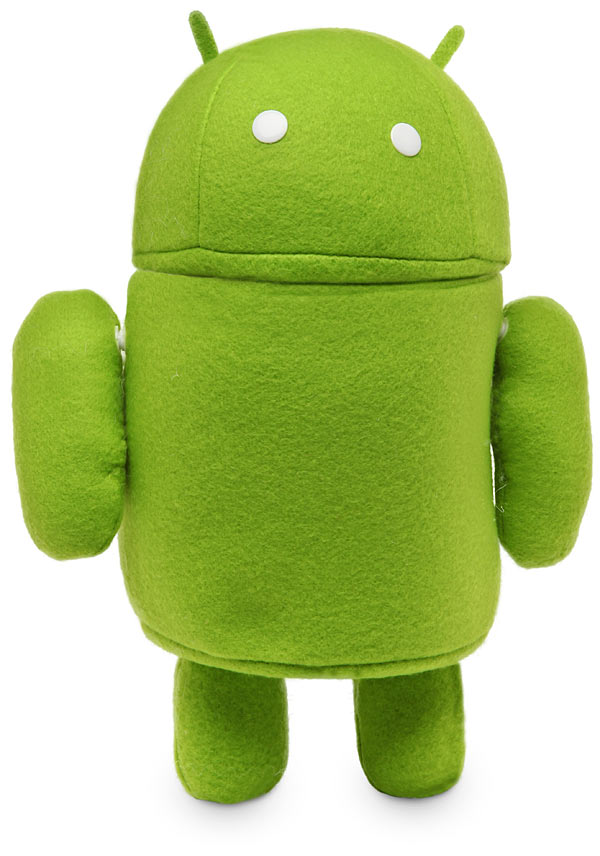
\includegraphics[width=5cm]{android_plush_robot.jpg}
	    \caption{Plain figure Plain figure Plain figure Plain figure Plain figure}
\end{figure}


\begin{figure}[htbp]
	\draftImage{width=5cm}{android_plush_robot.jpg}
	    \caption{Plain figure Plain figure Plain figure Plain figure Plain figure}
\end{figure}


\section{Kommunikationssysteme}
\blindtext
\subsection{TCP --- eine verbindundsorientierte Art}
\blindtext
\subsection{UDP --- verbindungslos}
\blindtext

\section{Verteilte Dateisysteme}
\blindtext

\section{Virtual Filesystem Switch (VFS)}
\blindtext

\section{Dateisystemschnittstelle FUSE}
\blindtext


\chapter{Anforderungen}


\chapter{Konzept und Design der Lösung}
\label{chap:Design}
\blindtext
\section{Konzept}

\begin{algorithm}
\DontPrintSemicolon
\KwData{$G=(X,U)$ such that $G^{tc}$ is an order.}
\KwResult{$G’=(X,V)$ with $V\subseteq U$ such that $G’^{tc}$ is an
interval order.}
\Begin{
$V \longleftarrow U$\;
$S \longleftarrow \emptyset$\;
\For{$x\in X$}{
$NbSuccInS(x) \longleftarrow 0$\;
$NbPredInMin(x) \longleftarrow 0$\;
$NbPredNotInMin(x) \longleftarrow |ImPred(x)|$\;
}
\For{$x \in X$}{
\If{$NbPredInMin(x) = 0$ {\bf and} $NbPredNotInMin(x) = 0$}{
$AppendToMin(x)$}
}
\nl\While{$S \neq \emptyset$}{\label{InRes1}
\nlset{REM} remove $x$ from the list of $T$ of maximal index\;\label{InResR}
\lnl{InRes2}\While{$|S \cap  ImSucc(x)| \neq |S|$}{
\For{$ y \in  S-ImSucc(x)$}{
\{ remove from $V$ all the arcs $zy$ : \}\;
\For{$z \in  ImPred(y) \cap  Min$}{
remove the arc $zy$ from $V$\;
$NbSuccInS(z) \longleftarrow NbSuccInS(z) - 1$\;
move $z$ in $T$ to the list preceding its present list\;
\{i.e. If $z \in T[k]$, move $z$ from $T[k]$ to
$T[k-1]$\}\;
}
$NbPredInMin(y) \longleftarrow 0$\;
$NbPredNotInMin(y) \longleftarrow 0$\;
$S \longleftarrow S - \{y\}$\;
$AppendToMin(y)$\;
}
}
$RemoveFromMin(x)$\;
}
}
\caption{IntervalRestriction\label{IR}}
\end{algorithm}

\subsection{Einsatz von FUSE} 

\subsection{Programminterne Darstellung von Dateibäumen}
	\label{sec:fsstruct}

\subsection{Client-Server Architektur}

\section{Programmablauf}

\section{Umgang mit Gerätedateien}


\section{Umgang mit Dateisystemrechten}
	\label{sec:permissions}

\chapter{Analyse der Applikation}

\chapter{Messungen und direkter Vergleich}
\label{sec:android}


\chapter{Schlussbetrachtung}
\section{Zusammenfassung}

\section{Fazit}

Auch die genannten Probleme aus Kapitel \ref{chap:Design} sollten in Zukunft berücksichtigt werden.

\subsection{Unterschiede zu bestehenden Lösungen}

\begin{table}[H]
	\begin{tabu} to \textwidth {l >{} X[l, 3] X[3] l}
		\tableHeaderStyle
		Aspekt & NFS & FUSE-Dateisystem \\
		Zugriffsmethode & Fernzugriffsmodel & Upload-/Downloadmodell \\
		Dateisystemmodell & uneingeschränktes UNIX-Dateisystemmodell & UNIX-Dateisystemmodell (ohne Unterstützung für symbolische Verknüpfungen, etc. Zudem können Dateien derzeit nicht erstellt werden, nachdem der Mount erfolgt ist. Diese Funktionalität ist dennoch leicht implementierbar. Gerätedateien können auch nicht angelegt werden)\\
		Kommunikation & betriebssystemunabhängige Client-/Serverkommunikation & betriebssystemunabhängige Client-/Serverkommunikation \\
		Prozesse & zustandloser Server & zustandsloser Server \\
		Namensraum & Unterschiedlicher Namensraum & Unterschiedlicher Namensraum \\
		Dateideskriptoren & serverseitig (eigenes Format) & clientseitig (UNIX-Format) \\
		Dateiattribute & 43 empfohlene Dateiattribute (laut NFS-Standard 4) & lediglich 6 \\
		Synchronisation & One-Copy Semantik (Unix) & Sitzungssemantik \\
		Dateisperren & werden über ein zusätzliches Protokoll (zustandsbehaftet) verwaltet. Es werden immer eine Reihe an Bytes gesperrt und keine ganzen Dateien. & Gibt es nicht; Letzter schreibender gewinnt. \\
		Caching & Einzelne Pakete werden zwischengespeichert & Ganze Dateien und deren Attribute werden zwischengespeichert. \\
		Rechteverwaltung & Access Control Lists & Keine
	\end{tabu}
	
	\caption[Vergleich zwischen FUSE-Dateisystem und NFS]{Vergleich zwischen FUSE-Dateisystem und NFS. Weitere Erläuterungen folgen unten.}
	\label{tbl:comparison}
\end{table}



\section{Defizite der Lösung}

\section{Ausblick}
Das entwickelte Protokoll könnte auf anderen Geräten wie in \cite{VERSYS} genutzt werden.

\chapter{Anhang}
\section*{Aufruf der Anwendung}

\listoffigures
\addcontentsline{toc}{chapter}{Abbildungs-, Programmcode- und Tabellenverzeichnis}
\lstlistoflistings 
\listoftables


%%% Referenzen %%%
%%% Wenn im Text nicht direkt referenziert, aber wichtig:
\nocite{MKLINUX}
\nocite{TANDISSYS}

\printbibliography 

\newgeometry{
  left=1cm,
  right=1cm,
  top=1cm,
  bottom=1cm,
  bindingoffset=5mm
}
\thispagestyle{empty}
\begin{center}
	\bfseries{\Large{Bewertung der \thesisType arbeit}}\\
\end{center}
\begin{center}
	\bfseries{\thesisTitle} von \thesisAuthor\\
\end{center}
\begin{center}
	\thesisSupervisor , am \today
\end{center}

\vspace{2ex}

\noindent{Qualität der Lösung: \textbf{Arbeitsweise und Lösungsweg}}
\begin{table}[H]
	\begin{tabu} to \textwidth {X[3,l] X[1,l] | X[1,l]}
       \tableHeaderStyle
        Kriterium & Selbsteinschätzung & Bewertung \\
	Zeiteinteilung des Studierenden & & \\
	Methodische Arbeitsweise & & \\
	Problemchen führt zum wochenlangen Abtauchen & & \\
	Aufteilung in Arbeitspakete & & \\
\end{tabu}
\end{table}
\begin{center}
	\platz{6}
\end{center}


\noindent{Qualität der Lösung: \textbf{Inhalt}}
\begin{table}[H]
	\begin{tabu} to \textwidth {X[3,l] X[1,l] | X[1,l]}
       \tableHeaderStyle
        Kriterium & Selbsteinschätzung & Bewertung \\
	Wurde das Problem angemessen gelöst & & \\
	Wurde etwas neues erreicht & & \\
	Passt der Umfang der Lösung zur Arbeitszeit & & \\
	Hinweise auf offene/ungelöste Probleme & & \\
	Nachvollziehbarkeit, Diskussion der eigenen Lösung? & & \\
	Wie viele Behauptungen werden nicht belegt/nicht bewiesen? & & \\
\end{tabu}
\end{table}
\begin{center}
	\platz{6}
\end{center}


\noindent{Qualität der Lösung: \textbf{Dokumentation und Ausarbeitung}
\begin{table}[H]
	\begin{tabu} to \textwidth {X[3,l] X[1,l] | X[1,l]}
       \tableHeaderStyle
        Kriterium & Selbsteinschätzung & Bewertung \\
	Lesbarkeit, Sprachstil und Verständlichkeit & & \\
	Systematik und roter Faden & & \\
	Passende Beispiele und Bilder & & \\
	Korrekte Zitierweise, passende Zitate & & \\
\end{tabu}
\end{table}
\begin{center}
	\platz{6}
\end{center}
\newpage
\thispagestyle{empty}

\noindent{Qualität der Lösung: \textbf{Implementierung}
\begin{table}[H]
	\begin{tabu} to \textwidth {X[3,l] X[1,l] | X[1,l]}
       \tableHeaderStyle
        Kriterium & Selbsteinschätzung & Bewertung \\
	Programmierstil, Lesbarkeit & & \\
	Weiterverwendung, Integrationsfähigkeit & & \\
\end{tabu}
\end{table}
\begin{center}
	\platz{6}
\end{center}


\noindent\textbf{Schwierigkeitsgrad} der Aufgabe
\begin{table}[H]
	\begin{tabu} to \textwidth {X[3,l] X[1,l] | X[1,l]}
       \tableHeaderStyle
        Kriterium & Selbsteinschätzung & Bewertung \\
	Verhältnis theoretischer zu praktischer Teil (bei geg. Aufgabe) & & \\
	Welcher Teil der Lösung war vorgegeben & & \\
	Nutzung von Wissen aus Lehrveranstaltung & & \\
	Wie formal bzw. mathematisch ist die Lösung? & & \\
\end{tabu}
\end{table}
\begin{center}
	\platz{6}
\end{center}


\noindent\textbf{Selbständigkeit} bei der Bearbeitung
\begin{table}[H]
	\begin{tabu} to \textwidth {X[3,l] X[1,l] | X[1,l]}
       \tableHeaderStyle
        Kriterium & Selbsteinschätzung & Bewertung \\
	Recherche, Arbeit mit Literatur/Bibliothek & & \\
	Eigene oder vorgeschlagene Lösungswege & & \\
	Regelmäßige Treffen, regelmäßiger Report & & \\
	Betreuungsaufwand (nicht selbständiges Arbeiten) & & \\
\end{tabu}
\end{table}
\begin{center}
	\platz{14}
\end{center}


\restoregeometry

\end{document}
